\documentclass[11pt]{article}

\usepackage{hyperref}
\usepackage{tikz}
\usetikzlibrary{snakes}

\title {{Functional requirements}}
\author {Lucie-Aim\'{e}e Kaffee}
\date{}

\begin {document}

  \section{Deployment cycles}
  Since there were different steps of deployments, it was necessary to split up the functional requirements and built up the requirements in every step on the ones before. \\
  The deployment timeline would look like this
  \\ 
  \\
    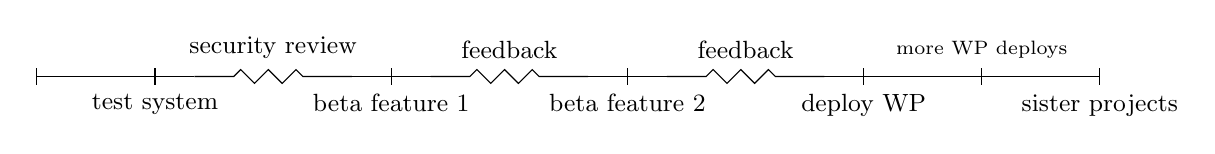
\begin{tikzpicture}[snake=zigzag, line before snake = 5mm, line after snake = 5mm]
      % draw horizontal line   
      \draw (0,0) -- (2,0);
      \draw[snake] (2,0) -- (4,0);
      \draw (4,0) -- (5,0);
      \draw[snake] (5,0) -- (7,0);
      \draw (7,0) -- (8,0);
	  \draw[snake] (8,0) -- (10,0);
	  \draw (10,0) -- (13.5,0);
      

      % draw vertical lines
      \foreach \x in {0,1.5,4.5,7.5,10.5,12,13.5}
	\draw (\x cm,3pt) -- (\x cm,-3pt);

      % draw nodes
      \draw (0,0) node[below=3pt] {} node[above=3pt] {$   $};
      \draw (1.5,0) node[below=3pt] {\small test system} node[above=3pt] {};
      \draw (3,0) node[below=3pt] {} node[above=3pt] {\small security review};
      \draw (4.5,0) node[below=3pt] {\small beta feature 1} node[above=3pt] {};
      \draw (6,0) node[below=3pt] {} node[above=3pt] {\small feedback};
      \draw (7.5,0) node[below=3pt] {\small beta feature 2} node[above=3pt] {};
      \draw (9,0) node[below=3pt] {} node[above=3pt] {\small feedback};
      \draw (10.5,0) node[below=3pt] {\small deploy WP} node[above=3pt] {};
      \draw (12,0) node[below=3pt] {} node[above=3pt] {\scriptsize more WP deploys};
      \draw (13.5,0) node[below=3pt] {\small sister projects} node[above=3pt] {};
    \end{tikzpicture}

  \subsection{Test system}
  To have a possibility to present the extension from the beginning, there was a test setup, available on \href{articleplaceholder.wmflabs.org/mediawiki}{wmflabs}. That test setup was specifically made to get a first idea of what the aims of the project are and was not intended to be used. 


  \subsection{security review}
  To deploy an extension to the Wikimedia cluster, it is necessary to have go through the process of the security review, usually done by the Wikimedia Foundation.

  \subsection{Beta feature}
  The next step was to deploy the extension as a beta feature. While having certain requirements for the test set up, the beta feature was supposed to be actually used by the community and therefore needed to fulfil more requirements, building up on what was already archived in the step before. \\
  After the first deploy as a beta feature, the feedback by the community needs to be evaluated and the extension needs to be adjusted accordingly. The adjusted beta feature needs not only to consider the feedback again but also to gain the support and trust of the community to be deployed on a Wikipedia.

  \subsection{Deploy to a Wikipedia}
  To deploy the extension on a Wikipedia, it is necessary to find a project, that would like to test the extension. Therefore, a ticket in the bug tracking system Phabricator was created. It asked for a Wikipedia to volunteer testing the extension live and provide feedback on how they liked it. \\
  To have it actually deployed, it must match more requirements and gain support by the local communities. The idea was, to deploy it on a Wikipedia, that has a limited amount of articles and maintainers, to actually see if it fulfils the needs of the readers it is aiming at. 

  \subsection{Deploy to more Wikipedias}
  It would be then necessary and possible to deploy it to more Wikipedias, that want to participate. 

  \subsection{Deploy to sister projects}
  In the future, it would be great to adjust the extension in a way that it's useful to other Wikimedia projects as well. This is out of the scope for the thesis but something to keep in mind while developing. 

 

\end {document}